\documentclass[../TDT5.tex]{subfiles}%

\begin{document}
\section{Étude d'un moteur de \textsc{Stirling}}
\enonce{%
	Le moteur de \textsc{Stirling} est constitué de deux chambres, une chaude et
	une froide, reliées par un régénérateur de volume constant pouvant être
	constitué de fils de cuivre tressés. Le gaz, en circuit fermé, reçoit un
	transfert thermique d’une source chaude (par exemple une chaudière à
	combustion) et cède un transfert thermique à la source froide (par exemple
	l’atmosphère).
	\smallbreak
	Le rôle du régénérateur, base de l’invention de Robert \textsc{Stirling}, est
	fondamental pour obtenir une bonne efficacité. Dans son brevet original de 1816,
	\textsc{Stirling} explique que le gaz chaud entre dans la partie chaude du
	régénérateur et est progressivement refroidi durant son parcours pour
	ressortir par l’autre extrémité à une température presque identique à la
	température de la source froide.
	\bigbreak
	Dans le parcours inverse, le gaz est progressivement réchauffé. Cette astuce
	technologique permet d’avoir une partie des échanges thermiques internes au
	moteur. On considérera le cycle parcouru par $n = \SI{40}{mmol}$ d’air,
	considéré comme un gaz parfait de rapport isentropique $\gamma = \num{1.4}$.
	\bigbreak
	Dans un premier temps, on néglige le régénérateur~: les deux chambres ne font
	qu’une. Le cycle de \textsc{Stirling} est alors modélisable par la succession de
	deux isothermes et deux isochores à partir d'un état 1 ($P_1 = \SI{1}{bar}$,
	$T_1 = \SI{300}{K}$). Il est décrit comme suit~:
	\begin{center}
		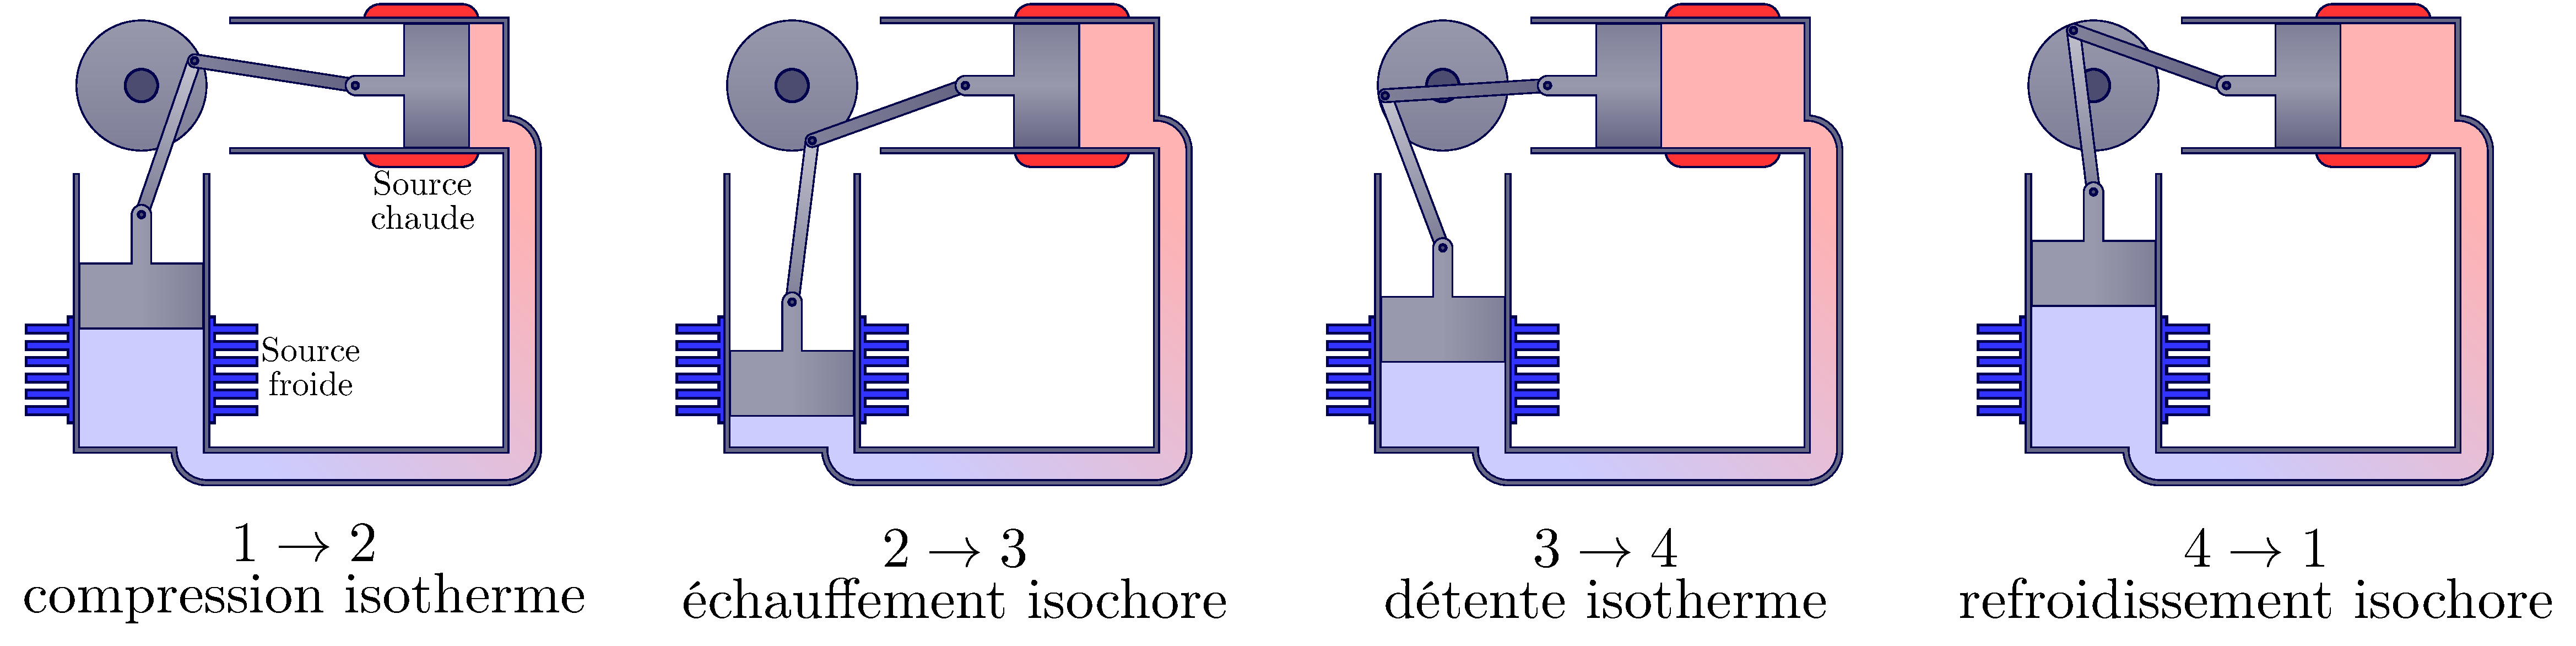
\includegraphics[width=\linewidth]{E4_schema_str}
	\end{center}
	\begin{itemize}
		\item $1\to 2$~: compression isotherme réversible à $T_F = T_1$ jusqu'à l'état
		      2, où $V_2 = V_1/10$~;
		\item $2\to 3$~: échauffement isochore au contact de la source chaude à $T_C =
			      \SI{600}{K}$ jusqu'à l'état 3 de température $T_3 = T_C$~;
		\item $3\to 4$~: détente isotherme réversible au contact de la source chaude à
		      $T_C$, jusqu'à l'état 4 de volume $V_4 = V_1$~;
		\item $4\to 1$~: refroidissement isochore au contact de la source froide
		      jusqu'à revenir à l'état 1.
	\end{itemize}
}%

\QR{%
	Calculer les valeurs numériques de $P,V,T$ pour chacun des quatre états.
}{%
	solu
}%

\QR{%
	Représenter ce cycle dans un diagramme de \textsc{Watt} (P,V). Justifier alors
	sans calculer que ce cycle est moteur.
}{%
	solu
}%

\QR{%
	Calculer pour chaque étape le travail et le transfert thermique reçus par le
	gaz. Commenter ces résultats~: a-t-on bien un cycle moteur~?
}{%
	solu
}%

\QR{%
	Quel est, sur le plan énergétique, la production de ce système sur un cycle~?
	Quel est le coût énergétique~? En déduire l'expression et la valeur du
	rendement.
}{%
	solu
}%

\QR{%
	Calculer l'entropie créée au sein du système au cours du cycle. Quel type
	d'irréversibilité entre en jeu~?
}{%
	solu
}%

\enonce{%
	L'invention du régénérateur par \textsc{Stirling} a permis d'améliorer
	considérablement le rendement de la machine précédente. Son idée est de faire
	en sorte que le gaz échange du transfert thermique au cours des
	transformations $2\to 3$ et $4\to 1$ non pas avec les thermostats, mais avec
	un système qui n'échange de l'énergie qu'avec les gaz au cours de ces
	transformations.
}%

\QR{%
	Justifier la pertinence de l'idée de \textsc{Stirling}.
}{%
	solu
}%

\QR{%
	Que vaut le rendement dans ces conditions~? Ce rendement peut-il être amélioré
	sans changer les sources~?
}{%
	solu
}%

% \begin{blocQR}
% 	\item \enonce{%
% 		En fonction des températures $T_F$ et $T_C$, du taux de compression $a =
% 			\frac{V_1}{V_2}$ et de $n$, $R$ et $\gamma$, établir les expressions~:
% 	}%
% 	\QR{%
% 	de la quantité de chaleur reçue par le système au cours d'un cycle
% 	(notée $Q_C$ et égale à $Q_{23}+Q_{34}$)~;
% 	}{%
% 	solu
% 	}%
%
% 	\QR{%
% 	de la quantité de chaleur cédée par le système au cours d'un cycle
% 	(notée $Q_F$ et égale à $Q_{41}+Q_{12}$)~;
% 	}{%
% 	solu
% 	}%
%
% 	\QR{%
% 		du rendement thermodynamique de ce cycle.
% 	}{%
% 		solu
% 	}%
%
% \end{blocQR}
%
% \QR{%
% 	On admet que la chaleur fournie au fluide lors du chauffage isochore est
% 	récupérée par un régénérateur lors du refroidissement isochore. Que devient
% 	le rendement~? Comparer ce rendement à celui de \textsc{Carnot}. Que peut-on
% 	en déduire sur l'entropie créée au cours du cycle~?
% }{%
% 	solu
% }%

\end{document}
